%%%%%%%%%%%%%%%%%%%%%%%%%%%%%%%%%%%%%%%%%
% This document provides a sample senior 
% thesis proposal template for use
% by Allegheny's Computer Science majors.
%
% This template was adopted from Jeremie Gillet
% Ref: https://github.com/oist/LaTeX-templates
%
% Author: Janyl Jumadinova
% Last Updated: 15 October 2021
%
%%%%%%%%%%%%%%%%%%%%%%%%%%%%%%%%%%%%%%%%%

%----------------------------------------------------------------------------------------
%	PACKAGES AND OTHER DOCUMENT CONFIGURATIONS
%----------------------------------------------------------------------------------------

\documentclass[12pt,oneside]{book} % 12 pt font, one-sided book style
\usepackage[a4paper, includehead, headheight=0.6cm, inner=3cm ,outer=2.5cm, top=2.5 cm, bottom=2.5cm]{geometry}  % Changing size of document
\usepackage[english]{babel} % The document is in English
\usepackage[utf8]{inputenc} % UTF8 encoding
\usepackage[T1]{fontenc} % Font encoding

\usepackage{graphicx} % For including images
\graphicspath{{./images/}} % Specifies the directory where images are stored

\usepackage{longtable} % tables that can span several pages
\usepackage[bf]{caption} % caption: FIG in bold
\usepackage{fancyhdr} % For the headers

\newcommand{\numberedchapter}{ % Preparation for numbered chapters
	\cleardoublepage % To make sure the previous headers are passed
	\fancyhead[RE]{{\bfseries \leftmark}}% Headers for left pages
	\fancyhead[LO]{{\bfseries \rightmark}}}% Headers for right pages
\newcommand{\unnumberedchapter}[1]{ % Preparation for unnumbered chapters
	\cleardoublepage % To make sure the previous headers are passed
	\addcontentsline{toc}{chapter}{#1} % Also adds the chapter name to the Contents
	\fancyhead[RE]{{\bfseries #1}} % Headers for left pages
	\fancyhead[LO]{}}%Headers for right pages

\usepackage{emptypage} % No headers on an empty page

\usepackage{eso-pic} % For the background picture on the title page
\newcommand\BackgroundPic{%
\put(0,-120){%
\parbox[b][\paperheight]{\paperwidth}{%
\vfill
\centering

\includegraphics[width=4in]{images/logo}%
\vfill
}}}

\usepackage{hyperref} % Adds clickable links at references

%----------------------------------------------------------------------------------------
%	ADD YOUR CUSTOM VALUES, COMMANDS AND PACKAGES
%----------------------------------------------------------------------------------------

% Open preamble/mydefinitions.tex and enter some values (name, thesis title...) 
% and include your own custom LaTeX functions and packages

%----------------------------------------------------------------------------------------
% values for the proposal
%----------------------------------------------------------------------------------------

\newcommand{\name}{Author Name} % Author name
\newcommand{\thesistitle}{Thesis Title} % Title of the thesis
\newcommand{\submissiondate}{\today} % Submission date "Month, date year"
\newcommand{\supervisor}{First Reader} % First reader's name
\newcommand{\cosupervisor}{Second Reader} % Second reader's name


%----------------------------------------------------------------------------------------
%	BIBLIOGRAPHY STYLE 
%----------------------------------------------------------------------------------------


\bibliographystyle{acm}

%----------------------------------------------------------------------------------------
%	YOUR PACKAGES (be careful of package interaction)
%----------------------------------------------------------------------------------------

\usepackage{amsthm,amsmath,amssymb,amsfonts,bbm}% Math symbols

%----------------------------------------------------------------------------------------
%	YOUR DEFINITIONS AND COMMANDS
%----------------------------------------------------------------------------------------

% New Commands
\newcommand{\bea}{\begin{eqnarray}} % Shortcut for equation arrays
\newcommand{\eea}{\end{eqnarray}}
\newcommand{\e}[1]{\times 10^{#1}}  % Powers of 10 notation


\begin{document}

%----------------------------------------------------------------------------------------
%	TITLE PAGE
%----------------------------------------------------------------------------------------

\pagestyle{empty} % No page numbers
\frontmatter % Use roman page numbering style (i, ii, iii, iv...) for the preamble pages

\begin{titlepage}
\AddToShipoutPicture*{\BackgroundPic}
\begin{center}
\vfill
{\large \scshape Allegheny College \\ Department of Computer Science }\\[1.4cm]
{\Large Senior Thesis}\\[0.5cm]
\rule{\textwidth}{1.5pt}\\[0cm]
{\huge \bfseries \thesistitle \par \ }\\[-0.5cm]
\rule{\textwidth}{1.5pt}\\[2.5cm]
\hfill  by\\[1cm]
\hfill  {\large \bfseries\name}\\
\vfill
{\hfill \large Project Supervisor: \textbf{\supervisor}} \\ 
\ifx\cosupervisor\undefined\else{\hfill \large Co-Supervisor: \textbf{\cosupervisor}} \\ \fi
\vspace{1cm}
\hfill  \submissiondate
\end{center}
\end{titlepage}


\pagestyle{fancy} % Changes the headers
\fancyhf{}% Clears header and footer
\fancyhead[RO,LE]{\thepage} % page number on the outside of headers

%-------------------------------------------------------------------------------
%	PREAMBLE PAGES (delete unnecessary pages)
%   preamble pages besides abstract are optional
%-------------------------------------------------------------------------------

\unnumberedchapter{Abstract} 
\chapter*{Abstract} 

Battery life of autonomous robots is vital to certain operations such as bomb
disposal or search and rescue. The longer a robot in those scenarios can operate,
the more likely it will be for them to potentially save lives. This project aims
to implement a tool that compares existing pathfinding algorithms and adds
additional evaluation metrics such as the expected energy cost of the selected
path, as well as the amount of memory required to run the algorithm. By comparing
the pathfinding algorithms with extra evaluation metrics, it should be possible to
obtain a more readily-applicable analysis of which algorithm will work best for a
specified environment type and/or a specified robot type. On top of the comparison
tool, this project will also implement a modified version of the A* algorithm that
will natively factor in energy cost when deciding on the optimal route for a robot
to take. This new algorithm will then be compared with the existing algorithms
using the tool created in this project. 

\unnumberedchapter{Acknowledgment} 
\chapter*{Acknowledgment} 

Theses should acknowledge assistance received in any of the following areas:

\begin{itemize}
\item Designing the research
\item Executing the research
\item Analyzing the data
\item Interpreting the data/research
\item Writing, proofing, or copyediting the manuscript 
\end{itemize}

\unnumberedchapter{Abbreviations} 
\chapter*{Abbreviations} 

\begin{longtable}{rl}
PACT & pathfinding algorithm comparison tool\\
\end{longtable}
\unnumberedchapter{Glossary} 
\chapter*{Glossary} 

% Break up this table into several ones if it takes up more than one page
\begin{center}
\begin{longtable}{r p{0.58 \textwidth}}
Dipole Blockade & Phenomenon in which the simultaneous excitation of two atoms is inhibited by their dipolar interaction. \\
Cavity Induced Transparency & Phenomenon in which a cavity containing two atoms excited with light at a frequency halfway between the atomic frequencies contains the number of photons an empty cavity would contain.  \\ 
\end{longtable}
\end{center}

\cleardoublepage
\thispagestyle{empty} % Page style needs to be empty for this page

\vspace*{8cm} 

\hfill
\begin{parbox}{0.6\textwidth}{
\begin{flushright}

If desired, an optional and short dedication may be included here.

\end{flushright}}
\end{parbox}




%-------------------------------------------------------------------------------
%	LIST OF CONTENTS/FIGURES/TABLES
%-------------------------------------------------------------------------------

\unnumberedchapter{Contents}
\tableofcontents % Write out the Table of Contents
\unnumberedchapter{List of Figures}
\listoffigures % Write out the List of Figures
\unnumberedchapter{List of Tables}
\listoftables % Write out the List of Tables

%-------------------------------------------------------------------------------
%	THESIS MAIN TEXT
%-------------------------------------------------------------------------------

\addtocontents{toc}{\vspace{2em}} % Add a gap in the Contents, for aesthetics
\mainmatter % Begin numeric (1,2,3...) page numbering

%----------------------------------------------------------------------------------------
%	START DELETE TEXT
%----------------------------------------------------------------------------------------

\section*{Template Overview}

You should first modify the documents in the preamble, things that appear before the main text as detailed below. 

\textbf{Front page}: use the one provided in this template, after changing the values like names in the file \texttt{preamble/mydefinitions.tex}.

\textbf{Abstract}: There should be a single paragraph of about 250 words, which concisely summarizes the entire proposal, written in the file \texttt{preamble/abstract.tex}.

\textbf{Acknowledgments, Abbreviations, Glossary, Dedication} preamble pages are optional and can be used at the author's discretion. 

The main text of the proposal should be stored in the ``SeniorThesis.tex'' document. The following descriptions are sections that must be included in the thesis document.

\textbf{Bibliography}: The bibliography should include all references cited in the text (as \cite{dasgupta2015comrade}) and it should not include references that have not been cited. ACM referencing style should be used when preparing the bibliography. We recommend using BibTeX or BibLaTeX and using the file \texttt{preamble/bibliography.bib}.

%----------------------------------------------------------------------------------------
% STOP DELETE
%----------------------------------------------------------------------------------------

%\numberedchapter{Introduction} % Title of the numbered chapter
\chapter{Introduction}
\label{ch:intro}

% This is the introduction. It should describe your completed senior thesis work, including the overall aims and the background motivating your research. Whenever possible, you should use one or more concrete examples
% and technical diagrams. 

% It is often useful and necessary to separate the introduction into multiple section. Several possible sections are proposed below, you can use these or distribute your introductory text into sections in another way. 

\section{Motivation} 
\label{sec:motivation}

% This section should include a statement of the problem, the overall aims, and the background motivating your research. Whenever possible, you should use one or more concrete examples
% and technical diagrams.
Pathfinding algorithms for autonomous field robots do not often take into account the energy cost of the path subsections when determining which route to traverse. This leads to wasted battery in robots where operational time is crucial to their intended purpose, like bomb disposal robots or search and rescue robots.\cite{henkel2016energy}. Robots that operate on battery and are sent into dangerous situations need to be able to operate for long enough that they can complete their mission without needing to come back and recharge. Many robots, such as bomb disposal robots, tend to waste power when traveling up inclines or on rough terrain, and this wasted power leads to a lower total operational time for the robot\cite{dasgupta2015comrade}.
\par
Longer operational time for field robots is a necessity, because in certain situations it can mean life or death for a person in a crisis. In search and rescue operations, such as in the case of natural disasters, people may be trapped and in imminent danger. The longer a robot can operate, the more likely it is that said person in danger can be located and/or rescued successfully. Another type of field robot that this affects is a bomb disposal robot. In post-conflict zones, the longer bombs are left, the more dangerous they become to the people in the region. Enabling each robot in the system to operate for longer means that in a given search, the robots are likely to find more bombs/explosives and deal with them properly\cite{dasgupta2015comrade}.
\par
A number of considerations are important when it comes to solving this problem, such as some of the following\cite{henkel2016energy}:
\begin{enumerate}
    \item Motor Resistance
    \item Friction
    \item System Vibrations
\end{enumerate}
\par
These elements all contribute to potential wasted power, because the higher the Motor Resistance, the more power it takes to move the motor a set distance. The more friction the ground exerts, the less power is required to rotate the wheels. The more friction the ball-bearings have in the wheels, the harder it is for the wheels to turn and thus it will draw more power. If the system is vibrating, then the ground friction will vary and a number of other issues with the robot will arise\cite{henkel2016energy}.

%\section{Current State of the Art}
%\label{sec:stateofart}
\section{Goals of the Project}
\label{sec:goals}
This project implements a simulation system that takes the pathfinding algorithms from several different sources and compares them in terms of different relevant metrics to the operational time of autonomous field robots. The intended functionality is for users to be able to provide or select from a few pathfinding algorithms currently used in autonomous field robots, and then the system designed in this project runs each of them and provides an analysis of how long each took to run, how much battery power the robot would require to traverse the chosen path, and also how much memory the algorithm used while it was running.
\par
This system provides the user with information about which algorithm is best suited to the robot that they provide as parameters to the simulation, and the expected environment in which that robot will operate. Each pathfinding algorithm will likely have certain environment types or robot weights in which cases they will be more effective and battery efficient. This research may also lead to a general case where a certain algorithm will be more efficient in most cases.
\par
By using this system, choosing the most battery-efficient pathfinding algorithm for the expected environment or the robot becomes easier, and enhances the operation time of autonomous robots in critical roles like search and rescue operations or bomb disposal. After this project, the simulation program will be able to be expanded for use with different pathfinding algorithms beyond those used in this project, and also with more complex sets of parameters and evaluation metrics for each algorithm.
\par
In addition to the simulation system, a modified version of the A* algorithm has been created that takes battery life into account as a weighting factor when determining the shortest path. Using the analysis of the other algorithms based on energy consumption, this new algorithm chooses a more energy efficient path than that of the other algorithms that do not inherently assess the energy cost of a given path. 

\section{Overview of Methods}
This project has created a "simulation room" of sorts in which a user is able to enter a pathfinding algorithm mathematically as a function, and compare it to other added robot pathfinding algorithms. This comparison is based on a variety of factors, such as the battery cost of the chosen route, the time it took to calculate the chosen route, and the amount of memory that was used during the calculation. The general process of using the simulation tool is outlined in Figure \ref{fig:Usage}.
\begin{figure}[H]
    \centering
    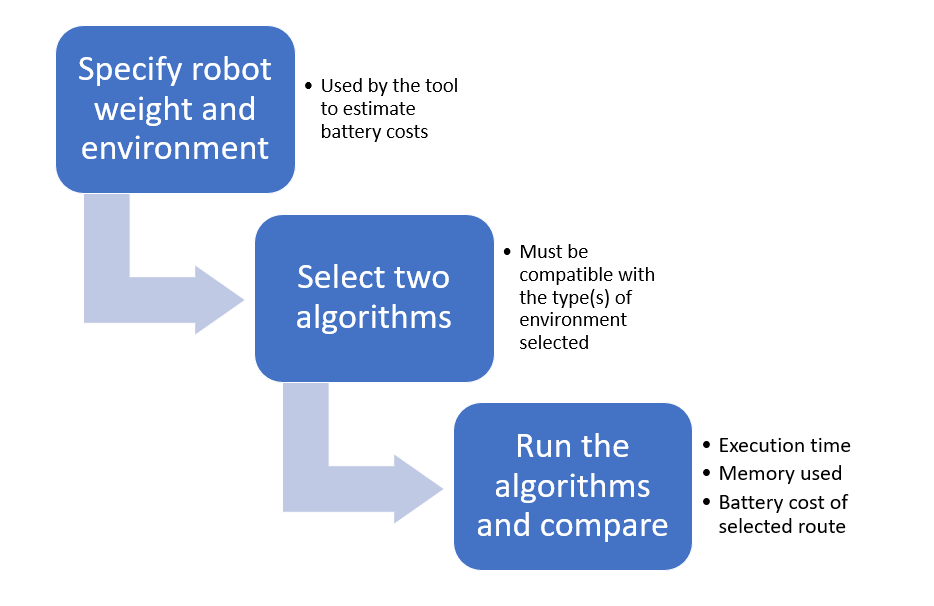
\includegraphics[width=5in]{../images/ProposalMethodFlowchart}
    \caption{The process for using the simulation tool}
    \label{fig:Usage}
\end{figure}
Each algorithm is able to be assessed based on the amount of time it takes to run the algorithm, how much memory it consumed, and how much battery power the calculated route will take to execute. Each of these metrics will be able to be used by robot designers to determine which algorithm best suits their needs for the robot that they are designing.
\par
This project has been written in Python due to the large number of available libraries and the general ease of use of the language. Numpy \cite{numpy_2021} has been used in the implementations of the various pathfinding algorithms, and the integrated system libraries were useful for tracking metrics such as the time it took to execute the algorithms and how much memory they use.
\par
As this approach purely looks at the performance of these pathfinding algorithms via a software approach and the physics used, the battery consumed statistic may be inaccurate when compared to a real robot using those pathfinding algorithms. Certain robot designs would likely require different amounts of battery power for a given route, meaning that in the future this system will likely need to be able to support different physics calculations based on varying numbers of drive motors or robot weights.
\par
This project assumes that each pathfinding algorithm will take either similar input or input that will be able to be derived from the simulated environment that will be created mathematically for traversal. Each pathfinding algorithm submitted for comparison will be tested with the robot type and environment held constant, such that the only variable changing on a comparison-by-comparison basis is which algorithm is being used and therefore also which path is selected for the robot to take to its objective.
\par
As for the inputs for the tool and for the new variant of the A* algorithm this project implemented, there will be several, as laid out in Table \ref{tab:inputs}.
\par
The Robot data is input as parameters ahead of the execution of the algorithms, as is the environment data. In the simulation tool, the other metrics regarding energy costs are calculated based on the output paths of the algorithms and combined to get an overall idea of the true battery cost of the algorithm. In the modified version of the A* algorithm, the energy cost metrics are  be calculated on a path-by-path basis during the execution of the algorithm.
\begin{table}[H]
\caption{Required attributes for the assessment of algorithms}\label{tab:inputs}
\centering
\footnotesize
\begin{tabular}{|l|l|l|l|}
\hline
\textbf{Attributes}          & \textbf{Data Type} & \textbf{Sample Value} & \textbf{Attribute Class}        \\ \hline
Battery Capacity                 & Decimal            & 2932.1                 & Robot Data               \\ \hline
Weight                           & Decimal            & 25.5                   & Robot Data               \\ \hline
Wheel Friction Coefficient       & Decimal            & 1.3                    & Robot Data               \\ \hline
List/Set of paths                & List               &                        & Environment Data         \\ \hline
Environment Friction Coefficient & Decimal            & 2.4                    & Environment Data         \\ \hline
Voltage                          & Decimal            & 1420.3                 & Electric Energy Cost   \\ \hline
Current                          & Decimal            & 1320.5                 & Electric Energy Cost   \\ \hline
Travel Time of Robot             & Decimal            & 35.6                   & Electric Energy Cost   \\ \hline
Velocity of robot                & Decimal            & 15.4                   & Friction Energy Cost   \\ \hline
Friction Coefficient(s)          & Decimal            & 3.1                    & Friction Energy Cost   \\ \hline
Distance Traveled                & Decimal            & 30.4                   & Friction Energy Cost   \\ \hline
Mass of robot                    & Decimal            & 43.2                   & Accel Energy Cost \\ \hline
Acceleration of robot            & Decimal            & 3.2                    & Accel Energy Cost \\ \hline
Distance Traveled                & Decimal            & 30.4                   & Accel Energy Cost \\ \hline
\end{tabular}
\end{table}

The pseudocode for the new algorithm is outlined in Algorithm \ref{alg:ModifiedA*}. This pseudocode is an altered version of the A* pseudocode presented by Akash\cite{akash_2020}. Each node's initial traversal cost is the raw distance needed to travel in meters for the robot, and the traversal costs are updated in the later half of the loop to factor in the energy cost of the given path as shown on line \ref{energyCostLine} of the algorithm.
\begin{algorithm}[H]
    \footnotesize
    \caption{Modified A* algorithm factoring in energy cost}\label{alg:ModifiedA*}
    \begin{algorithmic}[1]
        \State List of open nodes $\gets$ empty list
        \State List of closed nodes $\gets $ empty list
        \State OpenList $\gets$ StartNode
        \While{OpenList not empty}
            \State CurrNode $\gets$ node in OpenList with lowest (TravelCost + HeuristicValue)
            \State Remove CurrNode from OpenList
            \State Add CurrNode to ClosedList
            \If {CurrNode == Desired end node}
                \State Return path
            \EndIf
            \State CurrNodeChildren $\gets$ list of adjacent nodes to CurrNode
            \For{each child in CurrNodeChildren}
                \If{child is in ClosedList}
                    \State Skip to next iteration of this loop
                \EndIf
                \State child.TraversalCost $\gets$ CurrNode.TC + EnergyCostCalc(CurrNode.TC) + dist between CurrNode and child \label{energyCostLine}
                \State child.HeuristicVal $\gets$ Dist between child and end node
                \State child.TotalCost $\gets$ child.TC + Child.HeuristicVal
                \If{child.coords in OpenList nodes' coords}
                    \If{child.TC > OpenListNode.TC}
                        \State Skip to next iteration of this loop
                    \EndIf
                \EndIf
                \State Add child node to OpenList
            \EndFor
        \EndWhile
    \end{algorithmic}

\end{algorithm}

\section{Evaluation Strategy}
\label{sec:evaluate}

In this research, the primary means of evaluating each algorithm will be through the metrics of the amount of time it takes to calculate the most efficient path, the amount of memory on the device the algorithms use, and the amount of battery that traversing the chosen path will consume. Each algorithm is tested with a few different environments and robot weights, in an attempt to get the most full picture of the scenarios in which the algorithm functions the best. The processing steps are taking the inputs and feeding them into two different pathfinding algorithms in such a way that they obtain the same environment and robot data, so that the chosen path by each algorithm can be analyzed and compared based on total expected energy cost of the paths. During the execution of the algorithms, there are a few other metrics I capture such as the highest amount of RAM the algorithm uses, as well as the amount of time it takes for the algorithm to produce a valid result. 
\par
Automated software testing will be used to verify the accuracy of the calculations/features of the project. The Pytest \cite{pytest_2021} library will be used to run an automated test suite on the code developed in this project, making it easier to verify that the process by which the results are obtained is correct.
\par
Each metric used in comparing these pathfinding algorithms is used with simple algorithm/function examples such that their output can be guaranteed to be the expected value. Verifying the accuracy of metrics such as the amount of time it takes to run the function as well as the amount of memory a function uses helps to ensure that the analysis for the best algorithm is correct.
\par
The metric that is prioritized in this evaluation is the battery power cost of the route chosen by the algorithms. When choosing a pathfinding algorithm for autonomous field robots, depending on the task the robot is expected to perform, operational time can often be the limiting factor for them completing their task. By prioritizing minimization of battery costs, and weighing in the expected amount of time for the robot to traverse the path, it is possible to determine which algorithm will maximize the operational time of an autonomous robot.

% \section{Thesis Outline}
% \label{sec:outline} % Introduction (first numbered chapter)

%\numberedchapter{Related Work}
\chapter{Related Work} 
\label{ch:relatedwork}

%This chapter should include a broad and detailed review of relevant existing work. The literature review should provide background and context for the thesis work. The subsections may be organized in whatever
%manner seems best suited to the material---chronological, or by topic, or
%according to some other criteria (e.g., primary versus secondary resources).

Algfoor et al. \cite{abd2015comprehensive} provide an overview of pathfinding algorithms and how they convert real three-dimensional spaces into machine-traversable spaces. The representations of the environment that each algorithm takes can vary, from 2D or 3D grids to graphs or maps. Some algorithms use a waypoint system by which the robot breaks down its path into separate chunks based on pre-determined locations. There are also hierarchical approaches such as probabilistic roadmaps and random tree traversal. The most prevalent graph representation model for robotics pathfinding algorithms is a 2D square grid, and some of the algorithms that use these graphs are the Exhaustive and Monte-Carlo Iterative Taxing Algorithms and the Jump Point Search Algorithm. The Monte-Carlo algorithm relies on multiple calculation agents that randomly alternate once they reach an obstacle. An example of what one of these two-dimensional grids is provided by Jiang et al.\cite{jiang2018eight} in Figure \ref{fig:Environment}.
\begin{figure}[H]
    \centering
    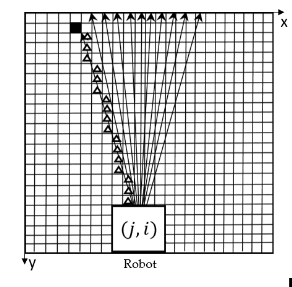
\includegraphics{images/EnvironmentRepresentation.PNG}
    \caption{Example environment representation}
    \label{fig:Environment}
\end{figure}
\section{Algorithm examples}
Bnaya et al. \cite{bnaya2013multi} present the Monte-Carlo Iterative Taxing Algorithm, which utilizes a few different software agents to traverse a 2-Dimensional grid. These software agents each can recognize when they would collide with either another agent or an obstacle, and they then must pay a “tax” in the form of waiting for an amount of time. By keeping track of all of these collisions, the algorithm constructs a series of "penalty tables" that store and compare the amount of tax paid per path found by the algorithm. The best path chosen by this algorithm will be the one with the lowest average sum of the penalty tables associated with the traversal.
\par
Karur et al. \cite{karur2021survey} discuss various extensions of the A* pathfinding algorithm, and therefore this resource can be used to great effect when implementing another version of the A* algorithm. The types of the A* algorithm discussed in this survey are shown in Table \ref{tab:algvariations}.
\begin{table}[H]\centering\footnotesize
    \caption{Variations of the A* algorithm presented by Karur et al.}\label{tab:algvariations}
    \begin{tabular}{|c|}
        \hline
        \textbf{A* Algorithm Variations} \\ \hline
        A* \\ \hline
        Hierarchical A* \\ \hline
        Hybrid A* \\ \hline
        Guided Hybrid A* \\ \hline
        A* with equal step sampling \\ \hline
        Diagonal A* \\ \hline
        A* with smart heuristics \\ \hline
        Lifelong Planning A* \\ \hline
    \end{tabular}
\end{table}
Using these other variants of the A* algorithm, it is possible to get a more full understanding of what different modifications will do to the basic A* algorithm. When this project makes its own version of the base A* algorithm, this context will be extremely useful in evaluating the effectiveness of the new algorithm.
\par
Vermette \cite{vermette2011survey} also discusses variations on the A* algorithm, which will provide even further context into what modifications can be made to the A* algorithm and how; in a very similar fashion to the Karur source listed previously.
\par
Belwariar's \cite{belwariar_2021} GeeksforGeeks article offers a solution for an implementation of the basic A* algorithm, and therefore can be used as a basis for my own understanding/implementation of the algorithm in this project. This algorithm takes in a grid of binary values (0 or 1) where a 0 means that the coordinate is non-traversable, whereas a 1 means it can be traversed. This type of grid can be used by my version of the A* algorithm, and stored in either a text file or a csv such that it can be easily imported to the simulation tool.
\par
Harabor and Grastien \cite{harabor2011online} designed an algorithm called the jump point search (JPS) algorithm which is an improvement on the A* algorithm. The JPS algorithm assesses all adjacent nodes in a 2D grid that are adjacent to the starting direction for each traversal. The algorithm uses "jump points" to limit the number of potential paths that the traversal needs to consider, therefore drastically reducing the amount of time it takes to arrive at the correct path for the robot/agent to take to its destination. Harabor and Grastien used the environment models proposed by Nathan R. Sturtevant \cite{sturtevant2012benchmarks} when testing their algorithm.
\section{Relevant Equations}
Henkel et al. \cite{henkel2016energy} developed a pathfinding algorithm that factors in the required battery power of each different path when making a decision on which it should take. This type of approach should be useful in informing how this proposed project can add battery power cost as an additional consideration for the autonomous robot, and therefore may be applicable to the A* algorithm that this project also aims to modify. This specific implementation of a pathfinding algorithm uses Djikstra's algorithm and the "Dynamic Window Approach" to simulate and choose from a number of possible trajectories for an autonomous field robot. In the end, the researchers concluded that their algorithm reduced the power consumption of an autonomous robot by almost ten(10) percent.
\par
Their algorithm factors in energy cost when considering routes to take\cite{henkel2016energy}, meaning that a similar approach can be used for calculating the energy required for other pathfinding algorithms. By analyzing the Electrical Energy, Frictional Energy, and Acceleration energy of the robot, it is possible to get an accurate projection by taking all of their sums. The Electrical Energy is calculated by taking the Voltage(U), the Current(I), and the time(t), and multiplying them together in this equation:\begin{equation}
    E_{et} = U\times I\times t
\end{equation}
Similarly, the Frictional Energy can be obtained by multiplying the velocity(v), the frictional coefficient(C), and the distance traveled(s):\begin{equation}
    E_{fric} = v \times C \times s
\end{equation}
And finally the Acceleration Energy can be calculated by multiplying the mass of the robot(m) with the acceleration(a) and the distance it travels(s):\begin{equation}
    E_{acc} = a \times m \times s
\end{equation}
These equations\cite{henkel2016energy} should be general enough to be applied to any robot and any pathfinding algorithm in order to get the energy required for a given path/trajectory.
\par
Li and Wang \cite{li2014coordinated} provide formulas for calculating the energy cost of wheeled robots attempting to climb slopes. In the proposal defense, there was a question raised about including topography in the calculations of energy cost along the ground. The equations presented in Li and Wang's paper, when included in the context of this project's algorithm comparison tool, are able to give a proper approximation of the true energy cost of traversing a slope with a wheeled robot. This approximation is used as a weight for the energy cost of traveling a given distance both in the modified A* algorithm constructed in this project, and in the comparison tool when calculating the energy cost of other algorithms.
\par The equations they use for calculating the traction efficiency of a six-wheeled robot are as follows:
    \begin{equation}
        T = F_{DP} \times l + F_{N} \times e
    \end{equation}
    \begin{equation}
        F_{DP} = \frac{T}{ r_{s}} - F_{N} \times \frac{e}{r_{s}}
    \end{equation}
Where T is 

%\numberedchapter{Method Of Approach}
\chapter{Method of Approach} 
\label{ch:method}

This chapter should answer the ``how'' question - how did you complete your project, including the overall design of your study, details of the algorithms and tools you have used, etc.  
 Use technical diagrams, equations, algorithms, and paragraphs of text to
describe the research that you have completed. Be sure to number all figures and tables and to explicitly refer to them in your text.


%\numberedchapter{Experimental Results}
\chapter{Experimental Results} 
\label{ch:experiments}

This chapter should describe your experimental set up and evaluation. It should also produce and describe the results of your study. Possible section titles are given below.

\section{Experimental Design}

\section{Evaluation}

\section{Threats to Validity}

%\numberedchapter{Conclusion}
\chapter{Discussion and Future Work}  
\label{ch:conclusion}

This is the conclusion. You might want to leave it unnumbered, as it is now. If you want to number it, treat it like any other chapter.

This chapter usually contains the following items, although not
necessarily in this order or sectioned this way in particular.

\section{Summary of Results}
A discussion of the significance of the results
and a review of claims and contributions.

\section{Future Work}

\section{Conclusion}


 
%----------------------------------------------------------------------------------------
%	BIBLIOGRAPHY
%----------------------------------------------------------------------------------------

\addtocontents{toc}{\vspace{2em}} % Add a gap in the Contents, for aesthetics
\unnumberedchapter{Bibliography} % Title of the unnumbered chapter
\bibliography{preamble/bibliography} % The references information are stored in the file named "bibliography.bib"


\end{document}  